\documentclass[preview]{standalone}

% tikz
\usepackage{tikz}
\usetikzlibrary{intersections, angles, quotes, positioning}
\usetikzlibrary{arrows.meta}
\usepackage{pgfplots}
\pgfplotsset{compat=1.13}
\tikzset{
	force/.style={thick, {Circle[length=2pt]}-stealth, shorten <=-1pt}
}

\begin{document}
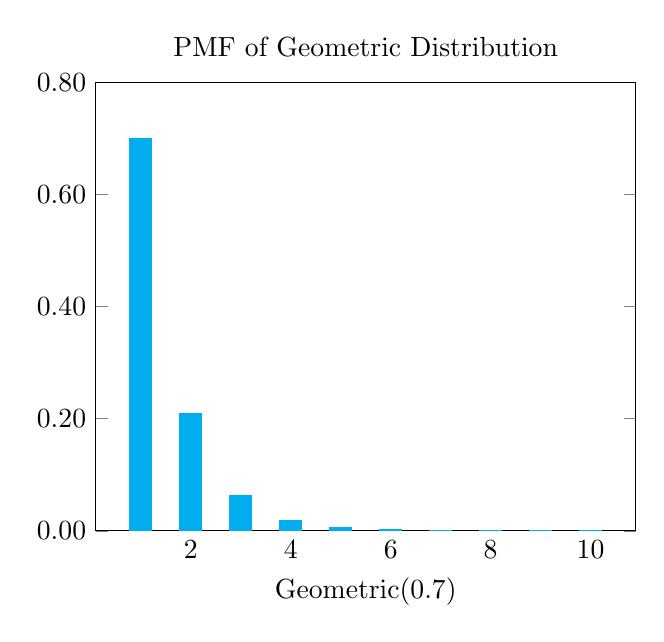
\begin{tikzpicture}
  \begin{axis}[
      title = {PMF of Geometric Distribution},
      ymin=0,
      ymax=0.8,
      xlabel = {Geometric(0.7)},
      samples at={1,...,10},
      xtick style={draw=none},
        yticklabel style={
            /pgf/number format/fixed,
            /pgf/number format/fixed zerofill,
            /pgf/number format/precision=2,
      },   
      domain=1:10,
      samples=10,
  ]
  % Define p, probability of success
  \pgfmathsetmacro{\p}{0.7}
  
  % Plot the PMF of the geometric distribution
  \addplot [
    ybar=0pt,
    bar width=8pt,
    fill=cyan,
    draw=cyan,
    mark=none,
] {(\p*(1-\p)^(x-1))};
  \end{axis}
  \end{tikzpicture}
\end{document}